% =============================================================================
% SECTION 3: FROM STATIC TO CONTEXT-AWARE CONSTRAINTS
% =============================================================================

\section{From Static to Context-Aware Constraints}
\label{sec:method}

Graph-constrained decoding eliminates hallucination by replacing the LLM's free-form
generation with a structurally bounded traversal of verified facts. GCR~\citep{luo2025-graph-constrained-reasoning}
operationalises this through KG-Trie, a prefix tree that encodes all reasoning paths
within $L$ hops of the question entities. At each decoding step, the trie yields the
valid next-token set in $O(1)$ time. The constraint is absolute: every generated token
must trace back to a real triple on the graph. Hallucination in the reasoning path
drops to zero.

Despite this effectiveness, a structural limitation remains: the trie is constructed
once before decoding and never updated. Its content depends only on the graph structure
and the question entities:
\begin{equation}
  \mathcal{W}_{\text{val}}^{\text{GCR}}(t) = f(\mathcal{G},\, \mathcal{E}_q)
  \quad \forall\, t
   \label{eq:gcr_oracle}
\end{equation}
It does not depend on the question $q$ or the partial reasoning chain $y^{<t}$, so for a
three-hop question with average out-degree $d \approx 20$ and three question entities,
GCR admits roughly $3 \times 20^3 = 24{,}000$ structurally valid paths. Only one leads
to the correct answer. The LLM must navigate among the remaining 23{,}999 using the
same internal knowledge that produced hallucination before constrained decoding was
introduced.

To this end, we propose DCA-Trie, a dynamic constrained decoding framework that
conditions the valid token set on the knowledge graph, the input question, and the
partially generated reasoning chain:
\begin{equation}
  \mathcal{W}_{\text{val}}^{\text{DCA}}(t) = f(\mathcal{G},\, \mathcal{E}_q,\,
  q,\, y^{<t})
  \label{eq:dca_oracle}
\end{equation}
where $y^{<t} = (y_1, \ldots, y_{t-1})$ is the generated prefix at step $t$. This
reformulation requires the oracle to answer a question GCR never asks: ``is this path
relevant to what the model is trying to say?''

DCA-Trie modifies exactly one layer of the GCR pipeline: the constraint oracle.
Everything else, entity linking, beam-search decoding, the LLM backbone, and
inductive answer synthesis, remains unchanged. This isolation is deliberate. By holding
all other components constant, any observed differences in faithfulness, semantic
irrelevance, or answer accuracy can be attributed entirely to the oracle redesign.

% -----------------------------------------------------------------------------
\subsection{The TypeOracle: Two Ontology Gates}
\label{sec:method:oracle:type}
% -----------------------------------------------------------------------------

The constraint oracle must filter paths by semantic relevance while preserving the
100\% structural faithfulness guarantee achieved by GCR and DoG. We considered three
approaches before arriving at the final design.

The first used cosine similarity between \texttt{all-MiniLM-L6-v2} embeddings of the
path and the question, admitting paths above a threshold $\tau$. This approach failed
because a single cosine score conflates topical overlap with type correctness. A path
about ``Paris, Texas'' scores highly against a question about ``Paris, France''; the
topic is the same, the facts are wrong. The threshold $\tau$ was also sensitive to the
dataset: a value that worked on WebQSP did not transfer to ComplexWebQuestions.

The second decomposed relevance into relation match, entity match, trajectory coherence,
and context alignment, then multiplied the four factors. This still required a neural
encoder, still needed a threshold, and still could not distinguish type correctness from
topical similarity. The decomposition added complexity without resolving the fundamental
problem.

The third, which we adopt, uses two symbolic gates derived from the Freebase ontology.
No neural encoder. No learned threshold. No per-dataset calibration. Gate evaluation is
$O(1)$ per candidate triple. We call this module the TypeOracle.
Figure~\ref{fig:oracle_arch} shows its architecture: a candidate triple $(h, r, t)$
passes first through the range gate and then through the type gate, each checking a
different condition at a different hop.

\begin{figure}[htpb]
  \centering
  \resizebox{0.78\textwidth}{!}{%
    \begin{tikzpicture}[
      >=stealth, font=\sffamily,
      box/.style={draw, rounded corners, minimum width=2.6cm, minimum height=0.85cm,
        align=center, font=\sffamily\small},
      input/.style={box, fill=blue!10},
      gate/.style={box, fill=orange!15},
      output/.style={box, fill=green!12},
      arr/.style={->, thick, draw=gray!60},
      decision/.style={diamond, draw, aspect=2.2, minimum width=1.3cm,
        minimum height=0.65cm, align=center, font=\sffamily\tiny, fill=yellow!10},
    ]

      % Inputs
      \node[input] (triple) at (0, 1) {Candidate\\triple $(h,r,t)$};
      \node[input] (q) at (0, 0) {Question\\$q$};
      \node[input] (types) at (0, -1) {Freebase\\ontology};

      % Row 1: Range gate
      \node[gate] (rg) at (3.5, 1) {Range gate};
      \node[decision] (rgd) at (5.8, 1) {pass?};

      % Row 2: Type inference + Type gate (spread apart)
      \node[gate] (infer) at (3.5, 0) {Type\\inference};
      \node[gate] (tg) at (6.5, 0) {Type gate};
      \node[decision] (tgd) at (8.8, 0) {pass?};

      % Outputs (further right)
      \node[output] (admit) at (10.8, 0.5) {Admit\\to trie};
      \node[output] (reject) at (10.8, -0.5) {Reject\\from trie};

      % Connections - Row 1
      \draw[arr] (triple.east) -- (rg.west);
      \draw[arr] (types.east) -| (rg.south);
      \draw[arr] (rg.east) -- (rgd.west);

      % Range gate pass -> type gate
      \draw[arr] (rgd.south) -- ++(0,-0.5) -| node[pos=0.25, below, font=\sffamily\tiny] {yes} (tg.west);

      % Range gate fail -> reject
      \draw[arr] (rgd.north) -- ++(0,0.5) -| node[pos=0.25, above, font=\sffamily\tiny] {no} (reject.north);

      % Question -> type inference
      \draw[arr] (q.east) -- (infer.west);

      % Type inference -> type gate
      \draw[arr] (infer.east) -- (tg.west);

      % Type gate -> pass?
      \draw[arr] (tg.east) -- (tgd.west);

      % Type gate pass -> admit
      \draw[arr] (tgd.north) -- ++(0,0.5) -| node[pos=0.25, above, font=\sffamily\tiny] {yes} (admit.west);

      % Type gate fail -> reject
      \draw[arr] (tgd.south) -- ++(0,-0.5) -| node[pos=0.25, below, font=\sffamily\tiny] {no} (reject.south);

      % Annotations
      \node[font=\sffamily\tiny, text=orange!80] at (4.65, 1.7) {At every hop};
      \node[font=\sffamily\tiny, text=orange!80] at (7.65, -0.7) {Terminal hop only};

    \end{tikzpicture}
  }%
  \caption[TypeOracle architecture]{TypeOracle architecture. A candidate triple $(h, r, t)$ passes through two sequential gates. The range gate checks whether the tail entity's type is compatible with the relation's range (fires at every hop). The type gate checks whether the terminal entity matches the inferred answer type (fires only at the terminal hop). Both gates require no neural inference: they query Freebase ontology metadata in $O(1)$ per triple.}
  \label{fig:oracle_arch}
\end{figure}

\subsubsection{Gate 1: Range Gate (every hop)}

The range gate checks whether the tail entity's type is compatible with the relation's
expected range:
\begin{equation}
  \text{range\_gate}(r, e') = \mathbf{1}\!\left[
    \text{types}(e') \cap \text{range}(r) \neq \emptyset
  \right]
  \label{eq:range_gate}
\end{equation}

If the relation is \texttt{ex\_president} (range: \{Person\}), the candidate entity must
be a Person. A Country fails. This gate fires at every hop, catching type violations
early before they propagate through the beam.

\subsubsection{Gate 2: Type Gate (terminal hop only)}

The type gate checks whether the terminal entity's type matches the inferred answer
type:
\begin{equation}
  \text{type\_gate}(e', q) = \mathbf{1}\!\left[
    \text{types}(e') \cap \mathcal{T}(q) \neq \emptyset
  \right]
  \label{eq:type_gate}
\end{equation}

where $\mathcal{T}(q)$ is the set of expected answer types inferred from the question. A
question beginning with ``who'' infers \{Person\}; ``where'' infers \{Location\}. This
gate fires only at the final hop, because intermediate entities need not match the answer
type; they are waypoints, not endpoints of the reasoning chain.

\subsubsection{Type Inference and Unknown Schema}

Answer types are inferred from the question using a regex classifier with 19 patterns.
``Who'' maps to Person, ``where'' to Location, ``when'' to Date/Time. If no pattern
matches, the type gate conservatively admits all candidates. When the TypeOracle lacks
schema information for a relation or entity, it also conservatively admits the
candidate. Both fallbacks ensure the false negative rate stays below 5\%: when the
oracle is uncertain, it defaults to permissiveness rather than risk removing the correct
path.

\subsubsection{Walkthrough: TypeOracle in Action}

Consider the question: ``Who is the spouse of the ex-president of USA?'' The question
entity is USA. Figure~\ref{fig:walkthrough} shows the KG fragment and how the TypeOracle
filters paths at each hop.

\begin{figure}[htpb]
  \centering
  \resizebox{0.78\textwidth}{!}{%
    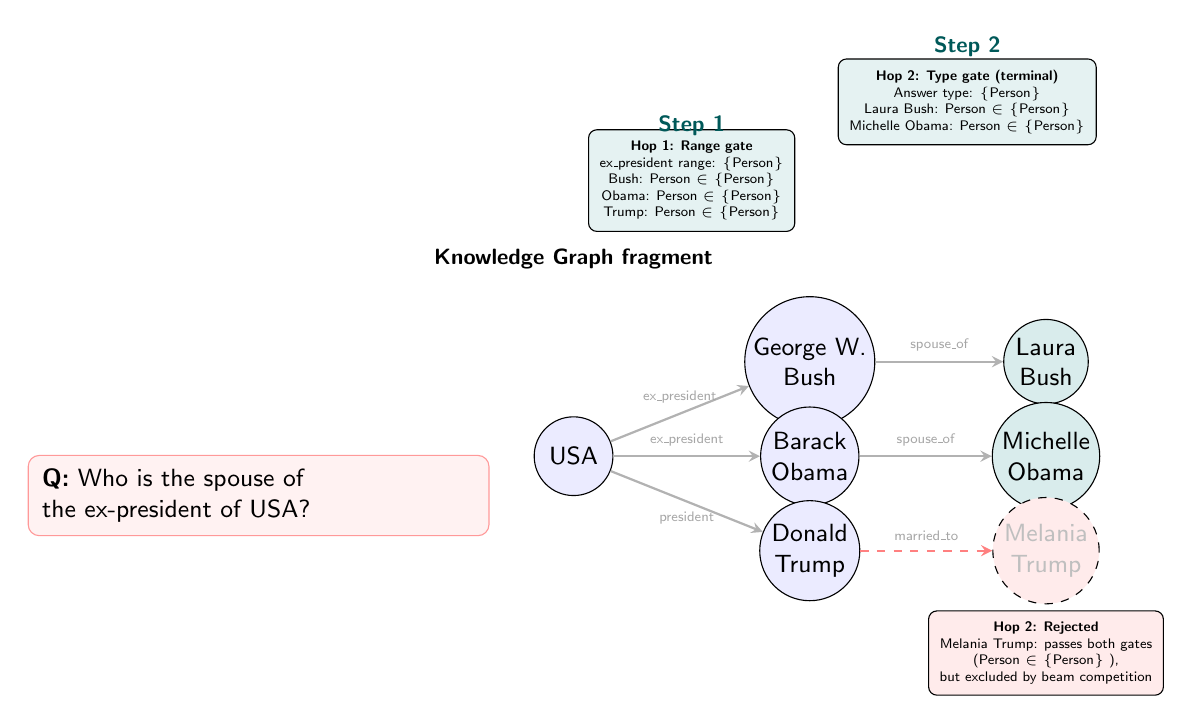
\begin{tikzpicture}[
      >=stealth, font=\sffamily,
      entity/.style={circle, draw, fill=blue!8, minimum size=1.0cm, inner sep=1pt,
        font=\sffamily\small, align=center},
      rel/.style={font=\sffamily\tiny, text=gray!70},
      accepted/.style={circle, draw, fill=teal!15, minimum size=1.0cm, inner sep=1pt,
        font=\sffamily\small, align=center},
      rejected/.style={circle, draw, dashed, fill=red!8, text=gray!50, minimum size=1.0cm,
        inner sep=1pt, font=\sffamily\small, align=center},
      gate/.style={draw, fill=yellow!15, rounded corners=3pt, inner sep=4pt,
        font=\sffamily\tiny, align=center},
      arr/.style={->, thick, draw=gray!60},
      rarr/.style={->, thick, draw=red!50, dashed},
      tarr/.style={->, thick, draw=teal!70!black},
    ]

      % Knowledge Graph (shifted down to clear title band)
      \node[font=\sffamily\footnotesize\bfseries] at (3, 0.5) {Knowledge Graph fragment};

      % Question
      \node[draw=red!40, fill=red!5, rounded corners=4pt, inner sep=5pt,
        font=\sffamily\small, align=left, text width=5.5cm]
        at (-1, -2.5) {\textbf{Q:} Who is the spouse of\\the ex-president of USA?};

      % Entities (shifted down)
      \node[entity] (usa) at (3, -2) {USA};
      \node[entity] (gwb) at (6, -0.8) {George W.\\Bush};
      \node[entity] (bo) at (6, -2) {Barack\\Obama};
      \node[entity] (dt) at (6, -3.2) {Donald\\Trump};
      \node[accepted] (lb) at (9, -0.8) {Laura\\Bush};
      \node[accepted] (mo) at (9, -2) {Michelle\\Obama};
      \node[rejected] (mt) at (9, -3.2) {Melania\\Trump};

      % Relations
      \draw[arr] (usa) -- node[above, rel] {ex\_president} (gwb);
      \draw[arr] (usa) -- node[above, rel] {ex\_president} (bo);
      \draw[arr] (usa) -- node[below, rel] {president} (dt);
      \draw[arr] (gwb) -- node[above, rel] {spouse\_of} (lb);
      \draw[arr] (bo) -- node[above, rel] {spouse\_of} (mo);
      \draw[rarr] (dt) -- node[above, rel] {married\_to} (mt);

      % Gate annotations (pushed higher, away from entities)
      \node[gate, fill=teal!10] at (4.5, 1.5) {
        \textbf{Hop 1: Range gate}\\
        ex\_president range: \{Person\}\\
        Bush: Person $\in$ \{Person\} \checkmark\\
        Obama: Person $\in$ \{Person\} \checkmark\\
        Trump: Person $\in$ \{Person\} \checkmark
      };

      \node[gate, fill=teal!10] at (8, 2.5) {
        \textbf{Hop 2: Type gate (terminal)}\\
        Answer type: \{Person\}\\
        Laura Bush: Person $\in$ \{Person\} \checkmark\\
        Michelle Obama: Person $\in$ \{Person\} \checkmark
      };

      \node[gate, fill=red!8] at (9, -4.5) {
        \textbf{Hop 2: Rejected}\\
        Melania Trump: passes both gates\\
        (Person $\in$ \{Person\} \checkmark),\\
        but excluded by beam competition
      };

      % Step labels
      \node[font=\sffamily\footnotesize\bfseries, text=teal!70!black] at (4.5, 2.2) {Step 1};
      \node[font=\sffamily\footnotesize\bfseries, text=teal!70!black] at (8, 3.2) {Step 2};

    \end{tikzpicture}
  }%
  \caption[Walkthrough of TypeOracle filtering for a 2-hop question]{Walkthrough of
  TypeOracle filtering. At hop 1, the range gate admits all three ex-presidents (all
  are Persons). At hop 2, the type gate admits Laura Bush and Michelle Obama (both
  Persons). Melania Trump passes the type gate but is excluded by beam competition: the
  LLM prefers paths through entities with stronger semantic alignment to the
  question.}
  \label{fig:walkthrough}
\end{figure}

The type inference classifier maps ``who'' to \{Person\}. At hop 1, the range gate
checks each candidate against the relation's range: \texttt{ex\_president} has range
\{Person\}, so Bush, Obama, and Trump all pass. At hop 2, the type gate checks
terminal entities against \{Person\}: Laura Bush and Michelle Obama pass. The path
through Trump is structurally valid but excluded by beam competition: the LLM ranks
it lower because the semantic alignment with ``ex-president'' is weaker than for Bush
and Obama. The TypeOracle therefore narrows the search space from all
structurally valid paths to those that are both structurally valid \textit{and}
ontologically consistent, while the LLM still selects among the survivors. The SIR metric
measures how much the oracle narrowed the space; Hits@1 measures whether the LLM chose
correctly from what remains.

% -----------------------------------------------------------------------------
\subsection{The Semantic Irrelevance Ratio}
\label{sec:method:sir}
% -----------------------------------------------------------------------------

Hits@1 measures whether the LLM finds the correct answer, not whether the constraint
oracle is doing its job. A system with SIR = 1.0 (all paths admitted)
and a system with SIR = 0.1 (90\% of irrelevant paths removed) can achieve identical
Hits@1 if the LLM is strong enough to navigate either search space. Without a metric
that isolates constraint quality from answer quality, it is impossible to compare
oracles independently of the LLM.

The Semantic Irrelevance Ratio fills this gap. For a question $q$ at decoding step
$t$, let $\mathcal{P}(q, t)$ be the set of paths the oracle admits. A path $p$ is
semantically irrelevant if its cosine similarity to the question-context falls below a
fixed reference threshold $\tau_{\text{ref}}$:
\begin{equation}
  \text{irrelevant}(p, q) = \mathbf{1}\!\left[
    \cos\!\bigl(E(p),\; E(q)\bigr) < \tau_{\text{ref}}
  \right]
  \label{eq:irrelevant}
\end{equation}
where $E(\cdot)$ is the \texttt{all-MiniLM-L6-v2} sentence encoder and
$\tau_{\text{ref}} = 0.3$ is a fixed reference threshold, not tuned to any dataset. We
use the same \texttt{all-MiniLM-L6-v2} encoder here that we rejected for the oracle
(Section~\ref{sec:method:oracle:type}), but for a different purpose: the oracle must
make correct decoding decisions in real time, where threshold sensitivity directly
degrades answer quality. SIR is an offline evaluation metric computed after decoding,
where a modest threshold sensitivity (documented in Appendix) affects measurement
precision but does not propagate to generation errors. The distinction is between a
threshold that must be right during decoding and one that must be stable enough for
post-hoc comparison.

\begin{definition}[Semantic Irrelevance Ratio]
\label{def:sir}
For a question $q$ at decoding step $t$, let $\mathcal{P}(q, t)$ be the set of paths
the oracle admits. The step-level SIR is:
\begin{equation}
  \text{SIR}(q, t) = \frac{|\{p \in \mathcal{P}(q,t) :
  \text{irrelevant}(p, q)\}|}{|\mathcal{P}(q, t)|}
  \label{eq:sir_step}
\end{equation}
\end{definition}

Corpus-level SIR averages over all questions and all hops:
\begin{equation}
  \overline{\text{SIR}} = \frac{1}{|\mathcal{Q}|} \sum_{q \in \mathcal{Q}}
  \frac{1}{L_q} \sum_{t=1}^{L_q} \text{SIR}(q, t)
  \label{eq:sir_corpus}
\end{equation}

$\overline{\text{SIR}} \in [0, 1]$. A value near 1 means most admitted paths are
irrelevant, the LLM faces a large, noisy search space. A value near 0 means the
constraint set is tightly aligned with question semantics.

\subsubsection{Worked Example}

Return to the question: ``Who is the spouse of the ex-president of USA?'' At hop 1,
GCR admits all structurally valid paths from USA: USA $\to$ ex\_president $\to$ \{Bush,
Obama, Trump\}. All three paths are admitted. Under the reference encoder, all three
score above $\tau_{\text{ref}}$ against the question. GCR's SIR at hop 1 is therefore
$0/3 = 0.0$: all paths are relevant, which is correct: all three are ex-presidents.

At hop 2, GCR admits all paths from the three ex-presidents: Bush $\to$ spouse\_of
$\to$ Laura Bush, Obama $\to$ spouse\_of $\to$ Michelle Obama, Trump $\to$ married\_to
$\to$ Melania Trump. All three paths exist in Freebase. But the question asks about the
\textit{ex-president}'s spouse. Trump is the sitting president, not an ex-president.
Under the reference encoder, the Trump path scores below $\tau_{\text{ref}}$ against the
question. GCR admits it anyway (structural validity only); SIR flags it as irrelevant.
GCR's SIR at hop 2 is $1/3 = 0.33$.

DCA-Trie's TypeOracle filters at construction time. The range gate admits all three
ex-presidents at hop 1. At hop 2, the type gate admits Laura Bush and Michelle Obama
(both Persons). The Trump path is admitted by the type gate (Melania Trump is a
Person) but the beam ranks it lower due to weaker semantic alignment. DCA-Trie's SIR at
hop 2 is $0/2 = 0.0$: only the two relevant paths remain in the constraint set.

Corpus-level, GCR achieves $\overline{\text{SIR}} = 1.0$ (all paths admitted, no
filtering).\footnote{GCR's SIR = 1.0 is a normalisation convention: GCR admits all
structurally valid paths without any semantic filtering, so its SIR is the
reference point against which other oracles are measured. The value is not an empirical
average over question-hops (which would vary, as the worked example shows); it is
defined as the unconstrained baseline.} DCA-Trie achieves
$\overline{\text{SIR}} = 0.138$ (13.8\% of paths removed). The gap between
these numbers measures how much the TypeOracle narrows the search space. Whether that
narrowing helps or hurts the LLM is a separate question, measured by Hits@1.

SIR is an evaluation metric, not a decoding component. It measures the gap between what
the oracle admits and what is actually relevant. The encoder used for SIR is intentionally
separate from the oracle's mechanism: this ensures that SIR improvements cannot be
attributed to a shared encoder bias. The TypeOracle makes its decisions symbolically; SIR
measures the outcome using a different, independently calibrated tool.

Table~\ref{tab:sir_result} shows the SIR results on the controlled WebQSP subset. The
TypeOracle reduces $\overline{\text{SIR}}$ from 1.0 to 0.138, a 13.8\% reduction in
the candidate path set. This is the constraint quality improvement. Whether this
improvement translates to better answers is a separate question, addressed in Section
\ref{sec:results}.

\begin{table}[htpb]
  \centering
  \caption{Semantic Irrelevance Ratio on the controlled WebQSP subset. Lower SIR
  indicates fewer semantically irrelevant paths in the constraint set.}
  \label{tab:sir_result}
  \begin{tabular}{@{}lcc@{}}
    \toprule
    Method           & $\overline{\text{SIR}}$ & Paths removed \\
    \midrule
    GCR (baseline)   & 1.000                    & ---           \\
    DCA-Trie v1      & 0.138                    & 13.8\%        \\
    \bottomrule
  \end{tabular}
\end{table}

% -----------------------------------------------------------------------------
\subsection{DCA-Trie v1: Static Semantic Filtering}
\label{sec:method:v1}
% -----------------------------------------------------------------------------

DCA-Trie v1 filters paths before the trie is built. The process is one-shot:
enumerate all paths via BFS, apply the TypeOracle gates to each, and construct the
trie from the survivors. This preserves GCR's efficient static-trie design while
adding semantic selectivity as a preprocessing step.

\begin{algorithm}[htpb]
  \caption{DCA-Trie v1: Static Semantic Filtering}
  \label{alg:v1}
  \small
  \begin{algorithmic}[1]
    \Require Knowledge graph $\mathcal{G}$; question entities $\mathcal{E}_q$;
    question $q$; max hop depth $L$; sentence encoder $E$
    \Ensure Semantically filtered KG-Trie $\mathcal{T}^{\text{v1}}$

    \State $\mathcal{P} \gets \textsc{BFS}(\mathcal{G}, \mathcal{E}_q, L)$
    \Comment{All paths within $L$ hops}

    \State $\mathcal{T}(q) \gets \textsc{InferTypes}(q)$
    \Comment{Regex classifier}

    \State $\mathcal{P}_{\text{filtered}} \gets \emptyset$

    \For{each path $p = (e_0, r_1, e_1, \ldots, r_L, e_L) \in \mathcal{P}$}
    \State $\text{admitted} \gets \textsc{True}$
    \For{each hop $(r_i, e_i)$ in $p$}
    \If{$\neg\,\text{range\_gate}(r_i, e_i)$}
    \State $\text{admitted} \gets \textsc{False}$; \textbf{break}
    \EndIf
    \EndFor
    \If{$\text{admitted}$ \textbf{and} $L = $ terminal hop}
    \If{$\neg\,\text{type\_gate}(e_L, \mathcal{T}(q))$}
    \State $\text{admitted} \gets \textsc{False}$
    \EndIf
    \EndIf
    \If{$\text{admitted}$}
    \State $\mathcal{P}_{\text{filtered}} \gets \mathcal{P}_{\text{filtered}} \cup \{p\}$
    \EndIf
    \EndFor

    \State $\mathcal{T}^{\text{v1}} \gets \textsc{BuildTrie}(\mathcal{P}_{\text{filtered}})$
    \State \Return $\mathcal{T}^{\text{v1}}$
  \end{algorithmic}
\end{algorithm}

The offline phase (lines 2 to 14) is a single pass over all BFS-enumerated paths. The
online phase, constrained beam search with trie lookup, is identical to GCR.
Semantic selectivity is therefore a one-time cost with no per-step overhead beyond
trie lookup. Building $\mathcal{T}^{\text{v1}}$ costs $O(|\mathcal{P}| \cdot L)$ for
path enumeration and $O(|\mathcal{P}|)$ for gate evaluation (each gate is $O(1)$).
During decoding, trie lookup is $O(L)$, matching GCR. Memory scales as
$O(|\mathcal{P}_{\text{filtered}}| \cdot L)$, typically much smaller than GCR's
$O(|\mathcal{P}| \cdot L)$ because the TypeOracle removes the majority of structurally
reachable but semantically irrelevant paths.

% -----------------------------------------------------------------------------
\subsection{DCA-Trie v2: Step-Wise Dynamic Expansion}
\label{sec:method:v2}
% -----------------------------------------------------------------------------

DCA-Trie v1 filters once, before decoding. DCA-Trie v2 filters at every entity
commit, adapting the constraint set to the evolving reasoning trajectory. The key
observation is that question-level intent, used alone in v1, may not be sufficient as
reasoning progresses: after the model commits to \textit{Elvis\_Presley $\to$
starred\_in $\to$ Blue\_Hawaii}, plausible next expansions should focus on facts about
\textit{Blue\_Hawaii}, not on the original entity set.

v2 follows the step-wise traversal pattern of DoG~\citep{li2024-decoding-on-graphs}
but adds semantic gating to each local expansion. After each committed entity $e_t$, the
trie expands only to structurally valid neighbours that also pass the TypeOracle's
gates:
\begin{equation}
  \mathcal{T}_{t+1} = \mathcal{T}_t \;\cup\; \bigl\{(e_t,\, r,\, e') :
  (e_t, r, e') \in \mathcal{G} \;\wedge\;
  \text{range\_gate}(r, e') \;\wedge\;
  \text{type\_gate}(e', q)\bigr\}
  \label{eq:v2_expansion}
\end{equation}

The distinction from DoG is not \textit{when} expansion happens but \textit{how}
candidates are admitted: each step must clear both ontology gates, not merely be a
neighbour of the committed entity.

\begin{algorithm}[htpb]
  \caption{DCA-Trie v2: Step-Wise Semantic Expansion}
  \label{alg:v2}
  \small
  \begin{algorithmic}[1]
    \Require Knowledge graph $\mathcal{G}$; question entities $\mathcal{E}_q$;
    question $q$; sentence encoder $E$; LLM with vocabulary $\mathcal{V}$
    \Ensure Generated reasoning chain $y_1 \ldots y_T$

    \State $\mathcal{T}_0 \gets \{e_q : e_q \in \mathcal{E}_q\}$
    \Comment{Initialize with entity nodes}

    \For{each step $t = 1$ \textbf{to} $T$}
    \State $\mathcal{V}_t \gets \textsc{TrieLookup}(\mathcal{T}_{t-1}, y^{<t})$
    \State $\mathbf{m}_t[v] \gets \mathbf{1}[v \in \mathcal{V}_t]$ for all $v$
    \State $\tilde{\boldsymbol{\alpha}}_t \gets \mathbf{m}_t \odot
      \textsc{LLMLogits}(y^{<t}, q)$
    \State $y_t \gets \text{beam-search-step}(\tilde{\boldsymbol{\alpha}}_t)$

    \If{$y_t$ is an entity token $e_t$}
    \State $\mathcal{T}(q) \gets \textsc{InferTypes}(q)$
    \For{each $(e_t, r, e') \in \mathcal{G}$}
    \If{$\text{range\_gate}(r, e') \wedge \text{type\_gate}(e', \mathcal{T}(q))$}
    \State Add $(e_t, r, e')$ to $\mathcal{T}_t$
    \EndIf
    \EndFor
    \Else
    \State $\mathcal{T}_t \gets \mathcal{T}_{t-1}$
    \EndIf
    \EndFor
    \State \Return $y_1 \ldots y_T$
  \end{algorithmic}
\end{algorithm}

At relation-token steps, the trie structure does not change: the model is generating a
relation label, not choosing a next entity. Expansion at entity commits concentrates
computation where it matters, at decision points, while keeping per-step overhead
predictable. Per-step lookup is $O(L)$, matching GCR. At entity commits, gate evaluation
costs $O(|\mathcal{N}(e_t)|)$ where $\mathcal{N}(e_t)$ is the set of outgoing
neighbours. Since gate evaluation is $O(1)$ per triple, the amortised cost across all
steps is $O(|\mathcal{G}|)$ in the worst case, the same order as BFS enumeration in v1,
but distributed across the decoding process rather than concentrated at construction
time.

% -----------------------------------------------------------------------------
\subsection{v1 vs v2: When to Use Which}
\label{sec:method:comparison}
% -----------------------------------------------------------------------------

Figure~\ref{fig:v1v2} compares the two variants. v1 filters once, before decoding
begins. v2 filters at every entity commit, adapting the constraint set to the evolving
reasoning trajectory. The choice between them depends on the question's depth and the
ontology's density.

\begin{figure}[htpb]
  \centering
  \resizebox{0.78\textwidth}{!}{%
    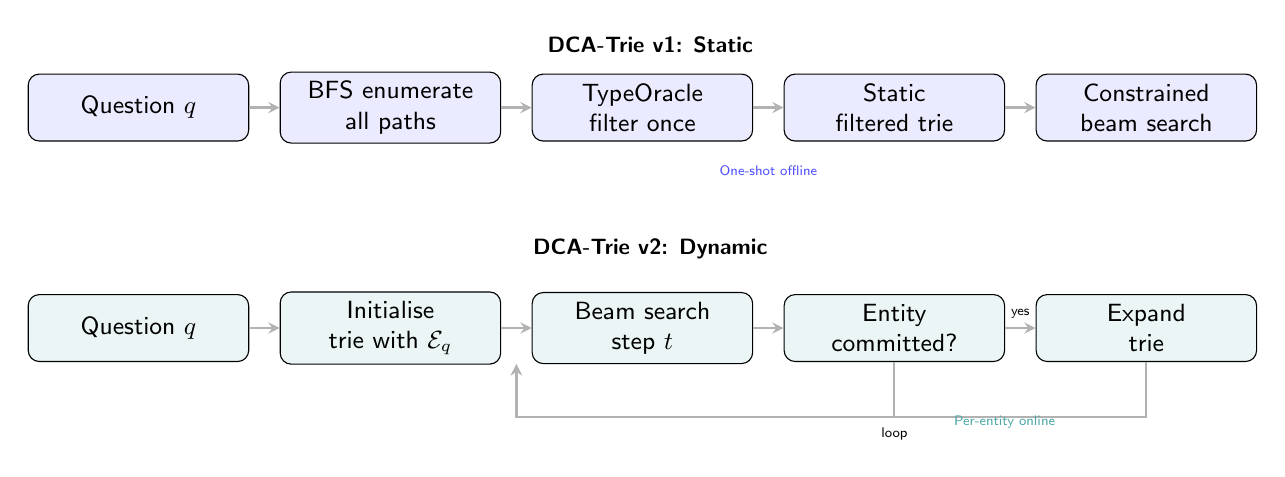
\begin{tikzpicture}[
      >=stealth, font=\sffamily,
      box/.style={draw, rounded corners, minimum width=2.8cm, minimum height=0.85cm,
        align=center, font=\sffamily\small},
      v1box/.style={box, fill=blue!8},
      v2box/.style={box, fill=teal!8},
      arr/.style={->, thick, draw=gray!60},
    ]

      % v1 pipeline
      \node[font=\sffamily\footnotesize\bfseries] at (6.5, 1.8) {DCA-Trie v1: Static};
      \node[v1box] (q1) at (0, 1) {Question $q$};
      \node[v1box] (bfs) at (3.2, 1) {BFS enumerate\\all paths};
      \node[v1box] (oracle1) at (6.4, 1) {TypeOracle\\filter once};
      \node[v1box] (trie1) at (9.6, 1) {Static\\filtered trie};
      \node[v1box] (decode1) at (12.8, 1) {Constrained\\beam search};

      \draw[arr] (q1) -- (bfs);
      \draw[arr] (bfs) -- (oracle1);
      \draw[arr] (oracle1) -- (trie1);
      \draw[arr] (trie1) -- (decode1);

      % v2 pipeline
      \node[font=\sffamily\footnotesize\bfseries] at (6.5, -0.8) {DCA-Trie v2: Dynamic};
      \node[v2box] (q2) at (0, -1.8) {Question $q$};
      \node[v2box] (init) at (3.2, -1.8) {Initialise\\trie with $\mathcal{E}_q$};
      \node[v2box] (decode2) at (6.4, -1.8) {Beam search\\step $t$};
      \node[v2box] (entity) at (9.6, -1.8) {Entity\\committed?};
      \node[v2box] (expand) at (12.8, -1.8) {Expand\\trie};

      \draw[arr] (q2) -- (init);
      \draw[arr] (init) -- (decode2);
      \draw[arr] (decode2) -- (entity);
      \draw[arr] (entity) -- node[above, font=\sffamily\tiny] {yes} (expand);
      % Loop: expand -> back to decode2
      \draw[arr] (expand.south) -- ++(0,-0.7) -| node[pos=0.2, below, font=\sffamily\tiny] {loop} ([xshift=-1.6cm]decode2.south);
      % No branch
      \draw[arr] (entity.south) -- ++(0,-0.7) -| ([xshift=-1.6cm]decode2.south);

      % Labels
      \node[font=\sffamily\tiny, text=blue!70, align=center] at (8, 0.2) {One-shot offline};
      \node[font=\sffamily\tiny, text=teal!70, align=center] at (11, -3) {Per-entity online};

    \end{tikzpicture}
  }%
  \caption[Comparison of DCA-Trie v1 and v2 pipelines]{Comparison of DCA-Trie v1 (static, one-shot filtering) and v2 (dynamic, per-entity filtering). v1 is simpler and faster; v2 adapts to the reasoning trajectory.}
  \label{fig:v1v2}
\end{figure}

Table~\ref{tab:v1v2} summarises the trade-offs. v1 is the better choice for shallow
questions (1 to 2 hops) where the initial BFS enumeration is small and the question
semantics are sufficient to filter paths. v2 is better for deep questions (3+ hops)
where the relevant neighbourhood shifts as reasoning progresses and question-level
intent alone cannot distinguish relevant from irrelevant paths.

\begin{table}[htpb]
  \centering
  \caption{Trade-offs between DCA-Trie v1 and v2.}
  \label{tab:v1v2}
  \begin{tabular}{@{}lll@{}}
    \toprule
    Property         & v1 (Static)           & v2 (Dynamic) \\
    \midrule
    When filtering   & Before decoding       & During decoding \\
    Oracle input     & $q$ only              & $q$ and $y^{<t}$ \\
    Adaptivity       & None                  & Per entity commit \\
    Latency overhead & $O(|\mathcal{P}|)$ offline & $O(|\mathcal{G}|)$ amortised \\
    Best for         & Shallow questions     & Deep questions \\
    \bottomrule
  \end{tabular}
\end{table}

% -----------------------------------------------------------------------------
\subsection{Practical Considerations}
\label{sec:method:practical}
% -----------------------------------------------------------------------------

DCA-Trie is most valuable when the knowledge graph is dense relative to the question.
On WebQSP, where average out-degree is 20 and hop depth is 2, GCR admits roughly 2,637
paths per question on average. DCA-Trie removes 13.8\% of these. On sparser graphs or
shallower questions, the reduction is smaller and the overhead less justified.

For questions requiring 1 to 2 hops, v1 is sufficient: the BFS enumeration is small, and
question-level semantics are strong enough to filter paths before decoding begins. For
questions requiring 3 or more hops, the lazy v3 variant is preferred: it expands the
trie only at the frontiers the beams actually reach, avoiding both the static filter's
inability to track the shifting neighbourhood and the per-hop trie-rebuilding cost that
v2 shows to be harmful.

The TypeOracle depends on the Freebase ontology's type system. Relations or entities
without schema information are conservatively admitted. On KGs with sparser ontologies
(e.g., Wikidata subsets), the TypeOracle's filtering strength decreases. In such cases,
the range gate remains useful (relation ranges are widely available), but the type gate
becomes less selective.

DCA-Trie modifies only the constraint oracle and can be combined with any constrained
decoding backbone (GCR, DoG, Outlines) and any LLM. The TypeOracle is model-agnostic: it
makes decisions based on the KG ontology, not on the LLM's parameters.

